\documentclass[14pt]{extarticle}
\usepackage{fontspec}
\usepackage{geometry}
\geometry{a4paper, margin=2.1cm}
\usepackage{graphicx}
\usepackage{booktabs}
\usepackage{array}
\usepackage{amsmath}
\usepackage{amssymb}
\usepackage[table]{xcolor}
\usepackage{titlesec}
\usepackage{fancyhdr}
\usepackage{enumitem}
\usepackage[most]{tcolorbox}

\definecolor{theme}{HTML}{2b6a77}
\definecolor{ink}{HTML}{232d33}
\definecolor{ok}{HTML}{3f8161}
\definecolor{warn}{HTML}{b5651d}
\definecolor{cardbg}{HTML}{f3f6f7}
\definecolor{softgray}{HTML}{eef1f2}

\setmainfont{THSarabunNew.ttf}[
  Path=./fonts/, BoldFont=THSarabunNew Bold.ttf,
  ItalicFont=THSarabunNew Italic.ttf, BoldItalicFont=THSarabunNew BoldItalic.ttf]
\setmonofont{cour.ttf}[Path=./fonts/, BoldFont=courbd.ttf, Scale=0.82]
\XeTeXlinebreaklocale "th"
\XeTeXlinebreakskip = 0pt plus 0.1pt

\titleformat{\section}{\Large\bfseries\color{theme}}{\thesection.}{0.5em}{}
\titleformat{\subsection}{\large\bfseries\color{ink}}{\thesubsection}{0.5em}{}
\setlist{itemsep=1pt, topsep=2pt}
\pagestyle{fancy}\fancyhf{}
\fancyhead[L]{\small\color{ink} CL-2 · Null / False-Positive Calibration}
\fancyhead[R]{\small\color{ink}\thepage}
\renewcommand{\headrulewidth}{0.4pt}
\newcommand{\code}[1]{{\ttfamily\detokenize{#1}}}
\newtcolorbox{keybox}{colback=cardbg, colframe=theme!55, boxrule=0.8pt, arc=2pt, left=8pt, right=8pt, top=5pt, bottom=6pt}

\begin{document}

\begin{center}
{\LARGE\bfseries\color{theme} รายงานการทดสอบสมมติฐาน CL-2}\\[3pt]
{\Large Null / False-Positive Calibration}\\[5pt]
{\small การตรวจจับรอยแตกด้วยลายเซ็นการกระเจิง (SPR) --- OpenGATE 10 / Geant4}\\
{\small รายงานเฉพาะการทดสอบ CL-2 (ด่านตรวจ validity) \quad$\bullet$\quad \today}
\end{center}
\vspace{2pt}{\color{theme!45}\hrule}\vspace{8pt}

\section*{บทคัดย่อ}
CL-2 เป็น\textbf{ด่านตรวจความถูกต้องของระเบียบวิธี} (validity gate) --- ตอบคำถามว่า
``a-priori ROI + multi-seed $t$-test สร้างผลบวกลวง (false positive) เมื่อไม่มีรอยแตกจริงหรือไม่''
ทดสอบ 3 วิธีบนข้อมูล CL-0 (ไม่ต้องรันใหม่): (1)~sign-flip permutation, (2)~control-vs-control,
(3)~spatial specificity ผลสรุป: \textbf{ระเบียบวิธี valid ทุกด่าน} --- อัตราผลบวกลวง
$=5.6\%/5.8\%\approx$ ค่าที่กำหนด $\alpha{=}5\%$, การตรวจพบยืนยันได้แบบ non-parametric, และ
\textbf{ไม่มี global artifact} $\Rightarrow$ การตรวจพบใน CL-0/CL-1 \textbf{เป็นของจริง มิใช่สิ่งประดิษฐ์ของ pipeline}

\section{สมมติฐานและขอบเขต}
\textbf{สมมติฐาน CL-2:} ระเบียบวิธีไม่สร้างสัญญาณลวงเมื่อไม่มีรอยแตก --- ถ้าถูกต้อง อัตราผลบวกลวง
ต้อง $\approx\alpha$ ($5\%$ ที่ระดับนัยสำคัญ $0.05$)\\
\textbf{ทำไมต้องทำก่อน:} ผลบวกทั้งหมด (การตรวจพบใน CL-0, ความเชื่อมั่นใน CL-1) ตั้งอยู่บนสมมติฐานว่า
การทดสอบมี calibration ถูกต้อง --- ถ้า false-positive rate สูง ผลบวกทุกอย่างจะน่าสงสัย
CL-2 จึงเป็น\textbf{ด่านตรรกะที่ต้องผ่านก่อน}เชื่อผลใด ๆ และวิเคราะห์ได้ทันทีจากข้อมูลที่มี

\section{วิธีวิเคราะห์ (3 การทดสอบอิสระ)}
\begin{enumerate}
  \item \textbf{Sign-flip permutation} (2.1): ภายใต้ null ป้าย ``fracture/control'' สลับกันได้
        $\Rightarrow$ พลิกเครื่องหมาย $\Delta$SPR ต่อ seed ทั้ง $2^8{=}256$ แบบ คำนวณ $t$ แต่ละแบบ
        $\to$ null distribution; empirical $p=$ สัดส่วนที่ $t\le t_{\text{observed}}$ (non-parametric)
  \item \textbf{Control-vs-control} (2.2): แทน ``fracture'' ด้วย control อีกชุด seed (แบ่งครึ่ง seed
        มาลบกันเอง) $\to$ ไม่มีรอยแตกจริง คำนวณ $p$ ที่ ROI ร่อง 5{,}000 การจับคู่
        $\to$ \textbf{FPR} $=P(p<0.05)$ และการกระจายของ $p$ (ควร uniform)
  \item \textbf{Spatial specificity} (2.3): สร้าง $t$-map ต่อพิกเซลทั้งลำแสง ดูว่าพิกเซลนัยสำคัญ
        \textbf{กระจุกที่ร่อง}หรือกระจายทั่ว (global artifact)
\end{enumerate}

\section{ผลการวิเคราะห์}

\begin{table}[h]\centering\small
\renewcommand{\arraystretch}{1.3}
\begin{tabular}{l c c c}
\rowcolor{softgray}
การทดสอบ & 0.306 มม. & 0.54 มม. & เกณฑ์ผ่าน \\
\midrule
2.1 sign-flip permutation ($p$) & 0.016 & 0.004 & $<0.05$ (มีนัยสำคัญ) \\
2.2 control-vs-control FPR & \textbf{5.6\%} & \textbf{5.8\%} & $\approx5\%$ \\
2.3 spatial (in-beam significant) & 4\% & 5\% & $\approx$ chance, กระจุกที่ร่อง \\
\bottomrule
\end{tabular}
\end{table}

\subsection{Null calibration --- อัตราผลบวกลวง $\approx5\%$}
เมื่อไม่มีรอยแตก (control-vs-control) การกระจายของ $p$-value \textbf{เกือบ uniform} และมีเพียง
$5.6\%/5.8\%$ ที่ $p<0.05$ --- \textbf{ตรงกับค่าที่กำหนด} $\alpha{=}5\%$ พอดี = การทดสอบ calibrate ถูกต้อง
ไม่เอนเอียงไปทางผลบวก

\begin{figure}[h]\centering
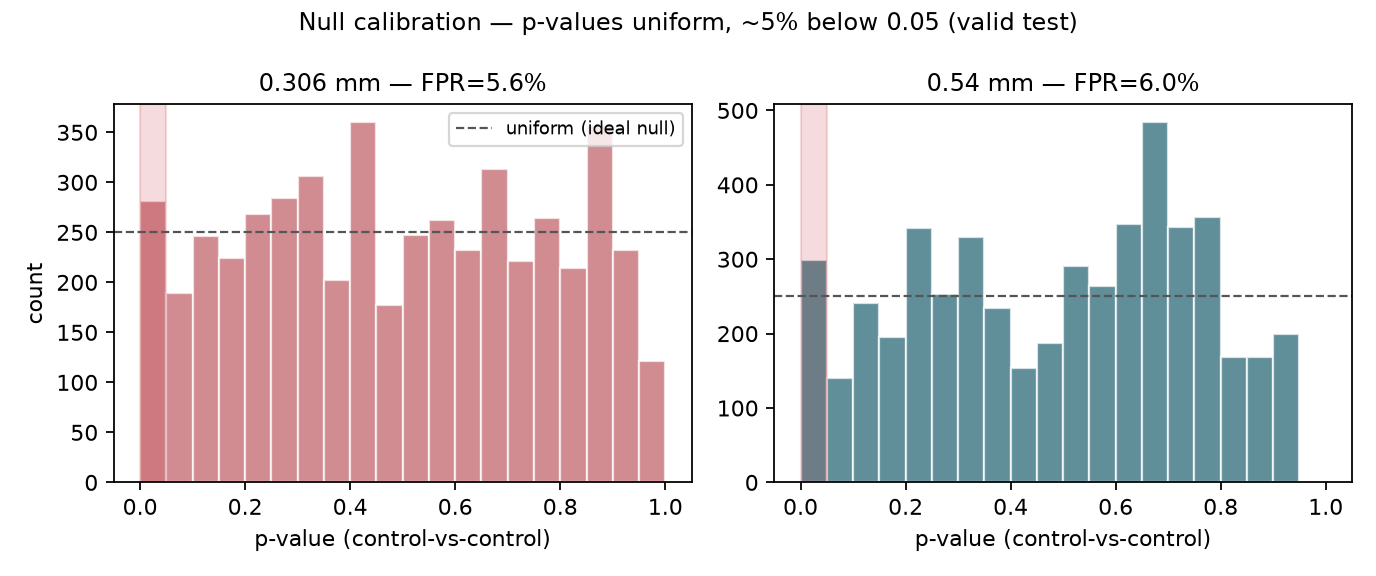
\includegraphics[width=0.90\textwidth]{fig_cl2/calib.png}
\caption{การกระจาย $p$-value ของ control-vs-control (ไม่มีรอยแตก) เกือบ uniform (เส้นประ = ค่าอุดมคติ);
แถบแดง = โซน $p<0.05$ ซึ่งมีเพียง $\sim$5\% ของกรณี = false-positive rate ปกติ}
\end{figure}

\subsection{Permutation --- การตรวจพบเป็นค่าสุดขั้ว}
$t$ ที่สังเกตได้ของร่องอยู่ที่\textbf{หางสุดขั้ว}ของ null distribution จากการพลิกเครื่องหมาย
(empirical $p=0.016$ ที่ 0.306~มม., $0.004$ ที่ 0.54~มม.) --- ยืนยันนัยสำคัญ\textbf{โดยไม่พึ่งสมมติฐาน
การแจกแจง $t$}

\begin{figure}[h]\centering
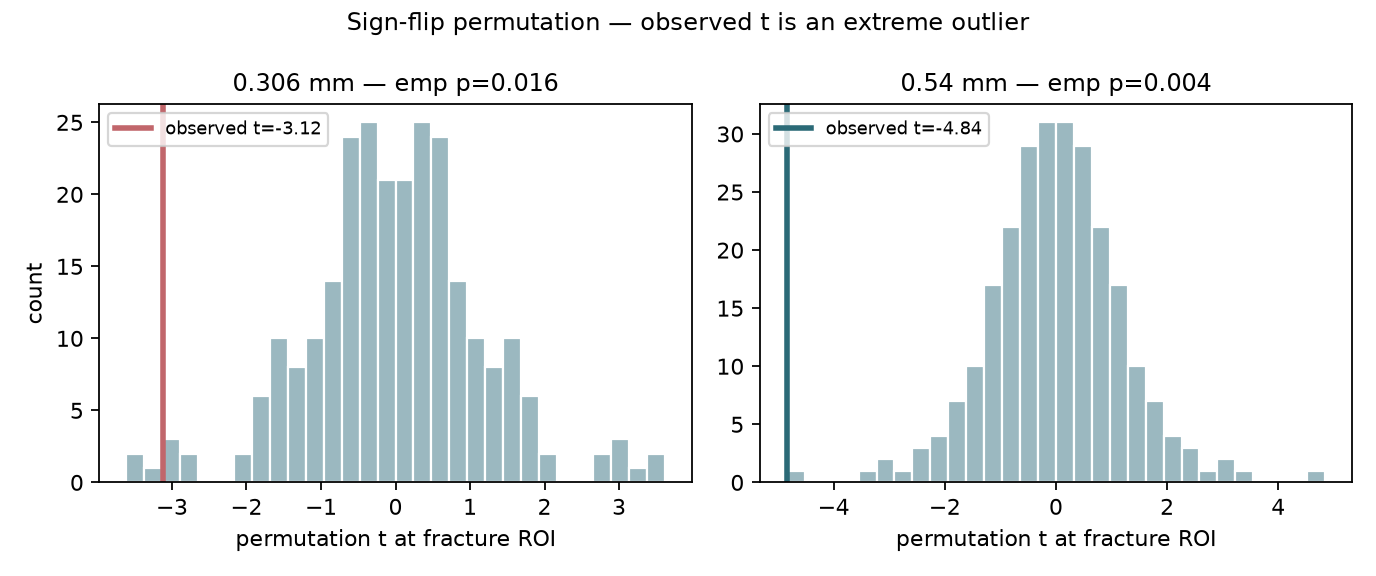
\includegraphics[width=0.90\textwidth]{fig_cl2/perm.png}
\caption{null distribution ของ $t$ จาก sign-flip permutation (256 แบบ); เส้นทึบ = $t$ ที่สังเกตได้จริง
ซึ่งอยู่ปลายหางซ้าย = การตรวจพบไม่ใช่ความบังเอิญ}
\end{figure}

\subsection{Spatial specificity --- ไม่มี global artifact}
ในลำแสง มีพิกเซลนัยสำคัญเพียง $4\%/5\%$ (\textbf{ระดับ chance} $\alpha{=}5\%$) และ\textbf{กระจุกใกล้ร่อง}
(ระยะเฉลี่ย $\sim$7--8px) มิได้สว่างทั้งลำแสง --- ยืนยันว่าการตรวจพบใน ROI-mean มิได้มาจากการเลื่อนระดับ
ทั้งภาพ (global offset) แต่เป็นสัญญาณเฉพาะที่ตำแหน่งร่อง

\begin{figure}[h]\centering
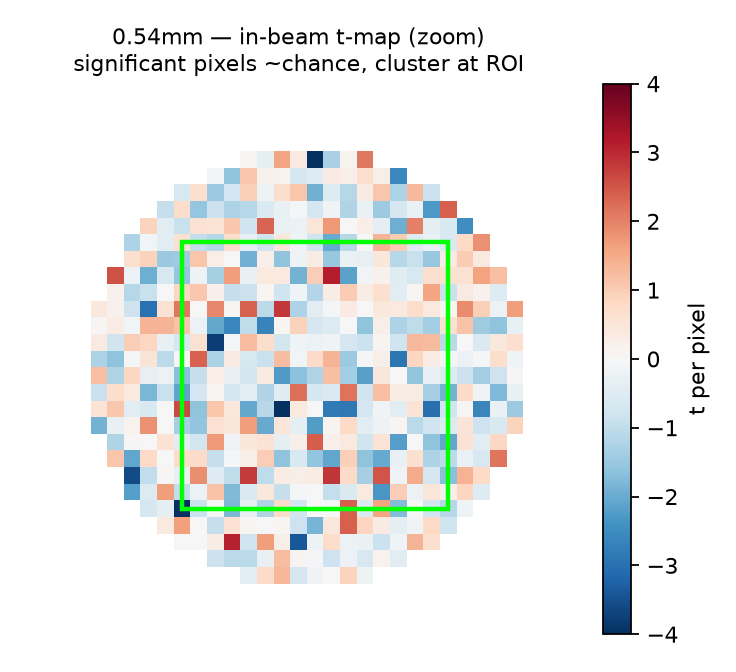
\includegraphics[width=0.52\textwidth]{fig_cl2/spatial.png}
\caption{$t$-map ต่อพิกเซลในลำแสง (0.54~มม., zoom); กรอบเขียว = ROI ร่อง พิกเซลนัยสำคัญอยู่ระดับ chance
และเกาะกลุ่มบริเวณร่อง ไม่กระจายทั่ว = ไม่มี artifact ทั้งภาพ}
\end{figure}

\section{สรุปการทดสอบสมมติฐาน CL-2}
\begin{keybox}
\textbf{ผลการทดสอบ:}\ \textcolor{ok}{$\boxtimes$ \textbf{ผ่านทุกด่าน --- ระเบียบวิธี valid}}\\[4pt]
เมื่อไม่มีรอยแตก ระบบให้ผลบวกลวงเพียง $\sim$5\% ตามที่การทดสอบระดับ $\alpha{=}0.05$ ควรเป็น;
การตรวจพบยืนยันได้แบบ permutation (ไม่พึ่งสมมติฐานการแจกแจง); และไม่มี global artifact
$\Rightarrow$ \textbf{การตรวจพบรอยแตกใน CL-0/CL-1 เป็นของจริง มิใช่สิ่งประดิษฐ์ของ pipeline หรือการเลือก ROI}
\end{keybox}

\section{นัยต่อการทดลองอื่น}
\begin{itemize}
  \item \textbf{ยืนยันความถูกต้องของ CL-0 และ CL-1 ย้อนหลัง} --- ผลบวกทั้งหมดผ่านด่าน validity แล้ว
  \item \textbf{De-risk การรัน 0.306~มม.\ @ \code{n_seeds=30}} --- เมื่อทราบว่า false-positive rate ปกติ
        การยกระดับ 0.306~มม.\ ให้ถึง $p<0.01$ จึงมีความหมาย (ไม่ใช่การไล่ตามผลลวง) $\to$ คุ้มที่จะรัน
  \item \textbf{a-priori ROI จำเป็น} --- spatial specificity ย้ำว่าต้องกำหนด ROI ที่ตำแหน่งร่อง\emph{ก่อน}
        ดูผล; การเลือก ROI จากจุดสว่างสุดจะเพิ่ม false positive
\end{itemize}

\vfill
\noindent{\color{theme!45}\rule{\textwidth}{0.4pt}}\\
{\small\color{ink} รายงานเฉพาะ CL-2 ประกอบ \code{report/methodology.pdf}. ตัวเลขทั้งหมดจากข้อมูล CL-0
(repository \code{GATE-Xray-pelvis-SPR}). ดู CL-1 = \code{report/cl1_report.pdf}, ผลฐาน = \code{report/report.pdf}.}

\end{document}
